\header{
    \headtitle{Le jeune homme de Besançon} \label{le-jeune-homme-de-besancon}
    %
    \insertComment{Publiée en 1911 dans Anthologie hospitalière et latinesque. Connue fin XIXe.}{}
}

\enluminure{4}{\href{https://www.youtube.com/watch?v=I3cqNOGWqMs}{U}}{n jeune} homme de Besançon \bissimple
\\Avait les poils du cul trop longs \bissimple
\\Il se retira pour les ton -on -on -on-dre
\\Dans un endroit obscur et som -om -om -om -bre
\\Comme il n'y voyait qu'à demi \bissimple
\\Il se coupa, un, deux trois
\\Le bout du vit! \} ter
\\\\Mécontent de c'qu'il avait fait \bissimple
\\Il prit les ciseaux qu'il tenait \bissimple
\\Et les jeta sur un' vieill' fem -em -em -em-me
\\Qui tout aussitôt rendit l'â -â -â -â-me
\\La justic' qui passait par là \bissimple
\\A êtr' pendu, un, deux trois
\\Le condamna! \} ter
\\\\Comme au supplice on le menait \bissimple
\\Et que le bourreau le tenait \bissimple
\\Il prit son vit à la poigné -é -é -é-e
\\Et le montra à l'assemblé -é -é -é-e
\\Le bourreau que cela fâcha \bissimple
\\Prit son couteau, un, deux trois
\\Et lui coupa! \} ter
\\\\Toutes les dames de la cour, \bissimple
\\De la ville puis des faubourgs, \bissimple
\\Prirent des pierr's en abondan -an -an -an-ce
\\Et les jetèr'nt avec violen -en -en -en-ce
\\Sur celui qui du jouvenceau, \bissimple
\\Avait réduit, un, deux trois
\\L'meilleur morceau! \} ter

\breakpage
Mais le plus beau d' cett' affair'-là, \bissimple
\\C'est que le bougre en réchappa \bissimple
\\Et baisa plus d'une da -a -a -a-me
\\En voulant lui prouver sa fla -a -a -a-mme
\\A la barbe d'un capucin \bissimple
\\Qui lui criait, un, deux, trois
\\Fils de putain. \} ter
\bigskip
\bigskip
\begin{center}
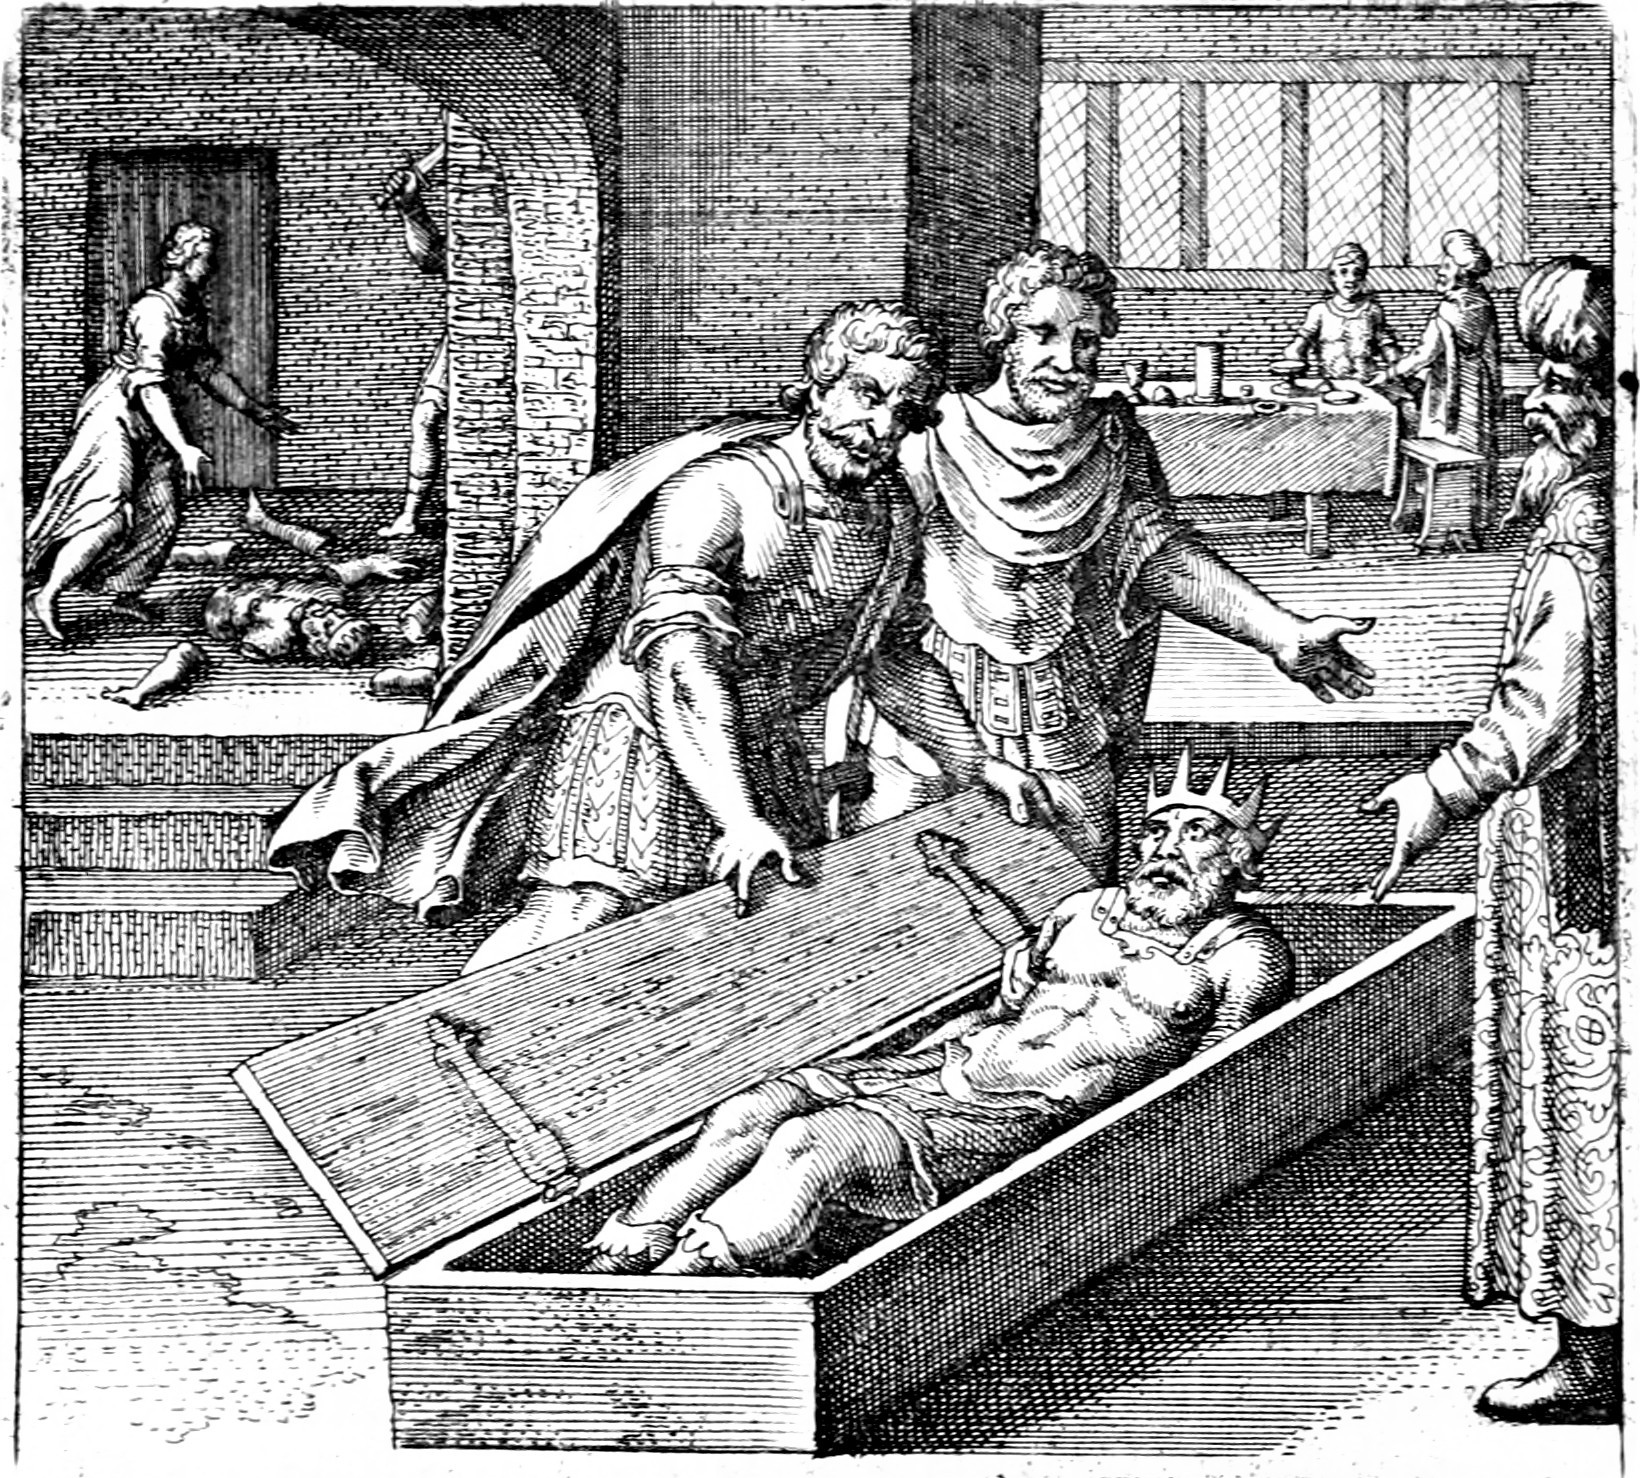
\includegraphics[width=1\textwidth]{images/brev58.png}
\end{center}
\breakpage